\documentclass[titlepage,10pt,a4paper]{article}
\usepackage[utf8]{inputenc}
\usepackage{graphicx}
\usepackage{hyperref}
\usepackage[ngerman]{babel}
\usepackage{float}
\usepackage{subcaption}
\usepackage{listings}
\usepackage{color}

\usepackage{glossaries}
\makeglossaries

\newglossaryentry{Server}{name={Server},
description={Der zentral ausgeführte Teil der Software, der die Kommunikation und
Interaktion mit den Clients verwaltet sowie erstellte Spiele verwaltet und
die Einhaltung der Regeln in diesen gewährleistet. }}

\newglossaryentry{Erstellungsfenster}{name={Erstellungsfenster},
description={Fenster, in welchem der Spielleiter die Eigenschaften des Spiels festlegt.}}

\newglossaryentry{Lobby}{name={Lobby},
description={Ort, an dem Spieler ein neues Spiel erstellen oder einem Spiel beitreten können.}}

\newglossaryentry{Regelwerk}{name={Regelwerk},
description={Ein bestimmtes Kartenspiel, bzw. die Regeln und Eigenschaften von diesem.}}

\newglossaryentry{Spielleiter}{name={Spielleiter},
description={Derjenige, der das Spiel erstellt hat.}}

\newglossaryentry{Wartefenster}{name={Wartefenster},
description={Fenster, in welchem man sich befindet, während man darauf wartet, dass die Mindestteilnehmerzahl erfüllt ist und das Spiel gestartet wird.}}

\newglossaryentry{Stich}{name={Stich},
description={Gewonnene Spielrunde.}}

\newglossaryentry{Spielrunde}{name={Spielrunde},
description={Eine Spielrunde endet, wenn jeder Spieler eine Karte gelegt hat.}}

\newglossaryentry{Partie}{name={Partie},
description={Eine Partie endet, wenn alle Karten gespielt wurden.}}

\newglossaryentry{Farbzwang}{name={Farbzwang},
description={Wenn man eine Karte der gleichen Farbe auf der Hand hat, wie die erste ausgespielte Karte, so muss diese gespielt werden.}}

\newglossaryentry{Trumpf}{name={Trumpf},
description={Die Farbe, die in der Runde am meisten Wert ist.}}

\newglossaryentry{IP-Adresse}{name={IP-Adresse},
description={Internet Adresse um der Server zu lokalisieren.}}

\title{Handbuch}
\date{\today{}, Passau}

\begin{document}
\begin{titlepage}
\vspace*{3cm}
\begin{center}
\textbf{\textsc{\LARGE Handbuch}}

{\large \today}

\vspace{2cm}
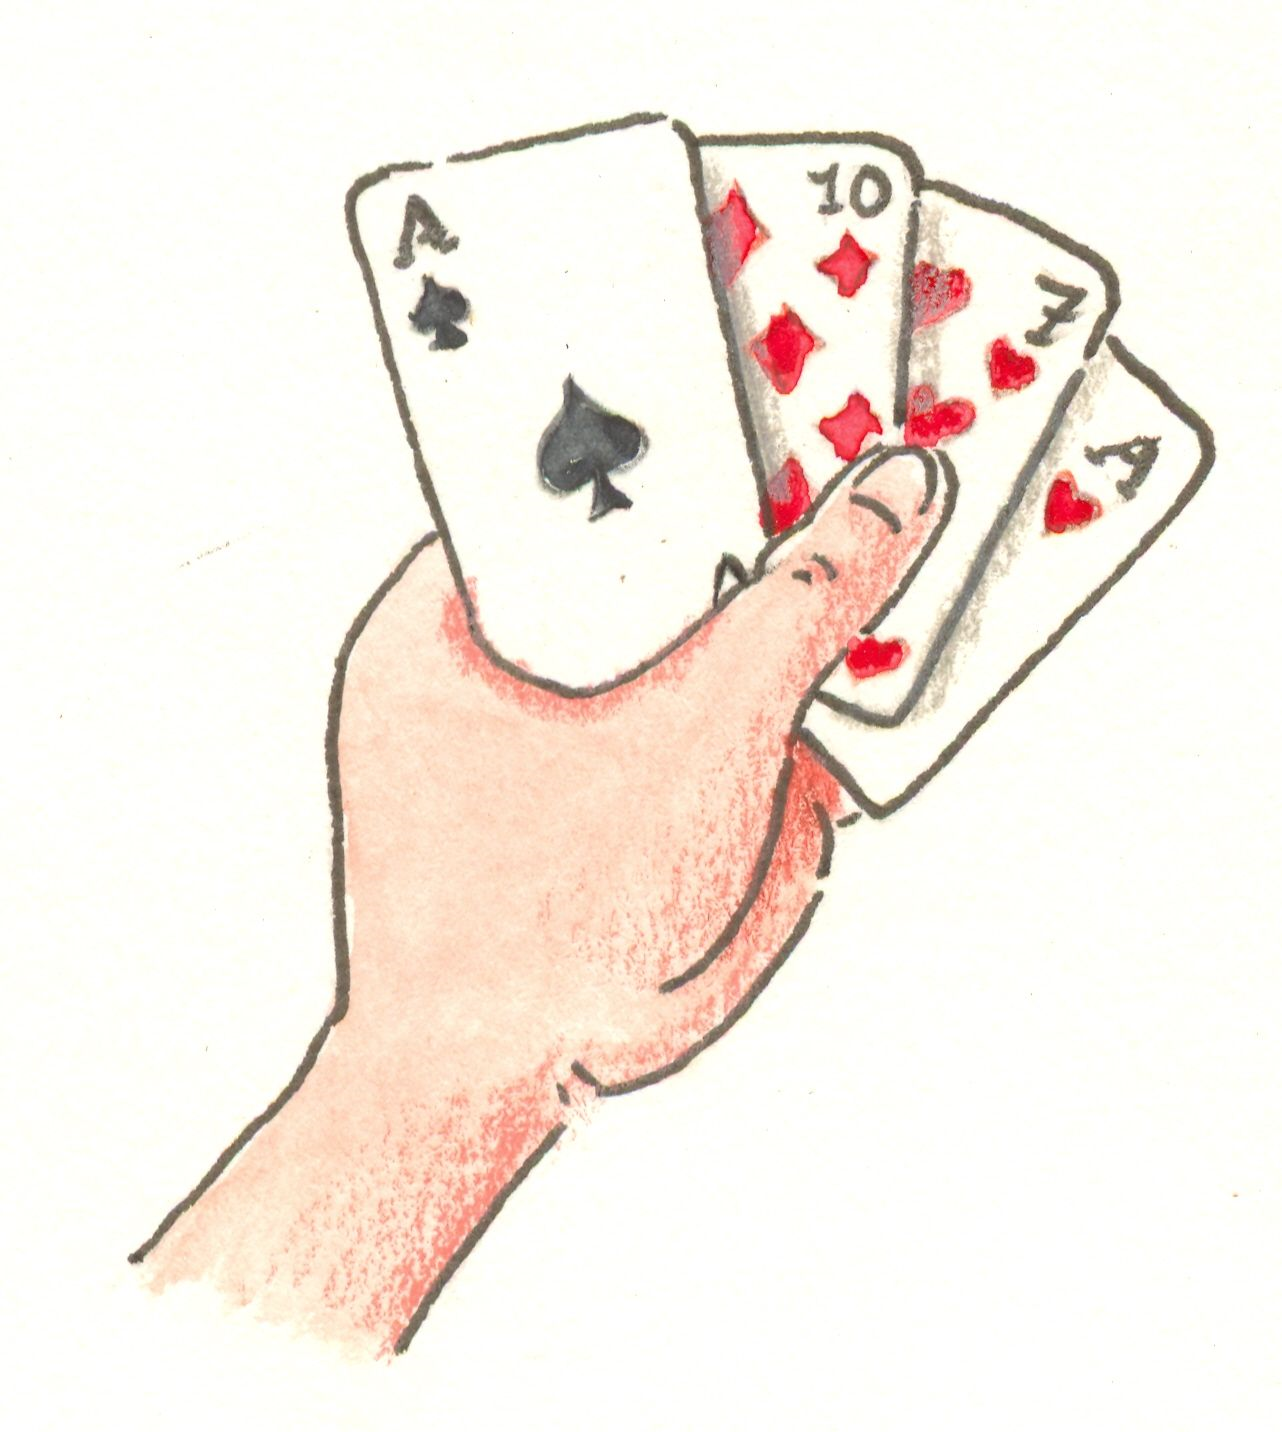
\includegraphics{kartenspiel}
\ \\
\ \\

\textbf{\textsc{\LARGE NET-WizHearts}}
\vspace{2cm}

\begin{tabular}{|c|c|c|}\hline
   Phase & Verantwortlicher & E-Mail \\ \hline\hline
   Pflichtenheft & Alina Meixl &  alina@meixl.de \\ \hline
   Entwurf & Viktoria Witka & witkaviktoria@freenet.de \\ \hline
   Spezifikation & Daniel Riedl & dariedl14@yahoo.de \\ \hline
   Implementation & Andreas Altenbuchner& a.andi007@gmail.com\\ \hline
   Validierung & Patrick Kubin & kubin@fim.uni-passau.de\\ \hline
   Präsentation & w& w\\ \hline
 \end{tabular}
\vspace{2cm}
\\
\end{center}
\end{titlepage}
\tableofcontents
\pagenumbering{arabic}
\hypersetup{pageanchor=true}

\newpage
 
\section{Einleitung}
Dies ist das Handbuch zum Spiel NET-WizHearts. NET-WizHearts ist ein Mulitplayer-Online-Kartenspielsystem, durch das mehrere Spieler über das Internet gegeneinander spielen können. Es gibt verschiedene Regelwerke, die gespielt werden können. Mitgeliefert werden bereits Hearts und Wizard. Die Anwendung ist so konzipiert, dass jederzeit weitere \gls{Regelwerk}e hinzugefügt werden können.

\section{Systemvoraussetzungen}
Dieses Produkt läuft auf den Betriebssystemen Microsoft Windows, Mac OS X und Linux. Java 7 Laufzeitumgebung muss vorhanden sein. Für das Spielen online ist ausserdem eine Internetverbindung vonnöten. \\
\gls{Server}seitig müssen zusätzlich die Mindestanforderungen des verwendeten Betriebssystems bezüglich Arbeitsspeicher und Rechenleistung erfüllt sein. Diese können durch die Anzahl der gehosteten Spieler/Spiele steigen.

\section{Installation}
Downloaden Sie die Datei NETWizHearts.rar und entpacken Sie diese. Es ist wichtig, dass der Ordner 'Data' am gleichen Ort abgelegt ist, wie die .jar Dateien. Kennen Sie bereits einen laufenden Server, so müssen Sie ausschließlich die NETWizHearts-Client.jar-Datei starten (siehe unten 'Spiel'). Möchten Sie selbst den Server stellen, beachten Sie den Punkt 'Server'.

\begin{itemize}
	\item \textbf{Server:} Mit Doppelklick auf die NETWizHearts-Server.jar-Datei starten Sie diesen.  Dazu muss das richtige Programm ausgewählt worden sein. Sollte dies nicht automatisch passiert sein und das Programm startet nach einem Doppelklick nicht, klicken Sie mit der rechten Maustaste auf die Datei -\textgreater Öffnen mit -\textgreater Standardprogramm auswählen -\textgreater Durchsuchen und wählen Sie dann die Datei javaw.exe unter folgendem Pfad aus: C:/Programme (x86)/Java/jre7/bin. \\
	Sie können das Programm auch aus der Konsole starten. Geben Sie hierzu in der Konsole ein: java -jar \textless Pfad zur Datei NETWizHearts-Server.jar\textgreater, dahinter können Sie optional eine Portnummer setzen, wenn Sie nicht den Standartport 4567 verwenden möchten, z.B.  java -jar \textless Pfad zur Datei NETWizHearts-Server.jar\textgreater 1234. \\
	Damit andere Mitspieler von außen auf den Server zugreifen können, müssen Sie den Port beim Router freigeben. Wie Sie diese Einstellungen vornehmen können, entnehmen Sie bitte der Gebrauchsanleitung Ihres Routers. Geben Sie nun den Port 4567 frei. Es kann auch ein anderer Port benutzt werden, allerdings muss der Server dann über die Konsole gestartet werden mit zusätzlicher Angabe der Portnummer, wie oben beschrieben.
	
	\item \textbf{Spiel:} Mit Doppelklick auf die NETWizHearts-Client.jar-Datei starten Sie das Spiel.  Dazu muss das richtige Programm ausgewählt worden sein. Sollte dies nicht automatisch passiert sein und das Programm startet nach einem Doppelklick nicht, klicken Sie mit der rechten Maustaste auf die Datei -\textgreater Öffnen mit -\textgreater Standardprogramm auswählen -\textgreater Durchsuchen und wählen Sie dann die Datei javaw.exe unter folgendem Pfad aus: C:/Programme (x86)/Java/jre7/bin. \\
	Sie können das Programm auch aus der Konsole starten. Geben Sie hierzu in der Konsole ein: java -jar \textless Pfad zur Datei NETWizHearts-Client.jar\textgreater.
	
	\item \textbf{Data:} Löschen Sie diesen Ordner nicht, benennen Sie diesen nicht um und verschieben Sie diesen nicht, sonst kann Ihr Spiel nicht mehr wie gewohnt angezeigt werden. Sollten Sie Bilder für den Hintergrund hinzufügen wollen, fügen Sie das Bild bitte in den Ordner 'backgrounds' ein. Sollten Sie Bilder für den Kartenhintergrund hinzufügen wollen, fügen Sie das Bild bitte in den Ordner 'cards' eins.
\end{itemize}

\section{Haftungsausschluss}
\begin{itemize}
\item \textbf{Haftung für den Inhalt} \\
Haftungsansprüche gegen den Autor, welche sich auf Schäden materieller oder ideeller Art beziehen, die durch die Nutzung des Programms verursacht wurden, sind grundsätzlich ausgeschlossen, sofern seitens des Autors kein nachweislich vorsätzliches oder grob fahrlässiges Verschulden vorliegt. 

\item \textbf{Urheberrecht} \\
Die Entwickler sind bestrebt, in dieser Anwendung die Urheberrechte anderer zu beachten bzw. nur auf selbst erstellte sowie lizenzfreie Werke zurückzugreifen.
Dieses Produkt unterliegt dem deutschen Urheberrecht. Beiträge Dritter sind als solche gekennzeichnet. Die Vervielfältigung, Bearbeitung, Verbreitung und jede Art der Verwertung der Inhalte außerhalb der Grenzen des Urheberrechtes bedürfen der Zustimmung der Ersteller. Dieses Produkt ist  nur für den privaten, nicht kommerziellen Gebrauch gestattet.

\item \textbf{Datenschutz} \\
Die Inanspruchnahme des angebotenen Dienstes ist ohne Angabe persönlicher Daten bzw. unter Angabe anonymisierter Daten oder eines Pseudonyms möglich.
\end{itemize}

\section{Spiel}
\subsection{Spielstart}
Bevor Sie die Anwendung starten können, müssen Sie sichergehen, dass ein \gls{Server} läuft. Um einen eigenen \gls{Server} zu starten, führen Sie die \gls{Server} JAR-Datei aus und geben Sie die gewünschte Portnummer in die Konsole ein. Bei leerer Eingabe wird ein Standardport verwendet. Zur Umsetzung siehe Punkt 3 'Installation - Server'. \\
Um das NET-WizHearts zu starten, führen Sie die Client JAR-Datei aus.  Zur Umsetzung siehe Punkt 3 'Installation-Spiel'.\\

\subsection{Einloggen}
Sobald Sie die Anwendung starten, sehen Sie als erstes das Login-Fenster. In diesem Fenster können Sie sich mit einem Benutzernamen anmelden und zu einem \gls{Server} verbinden. Außerdem können Sie auswählen, in welcher Sprache das Programm laufen soll.\\
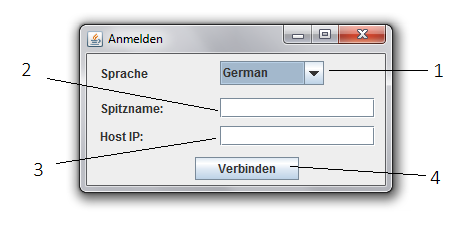
\includegraphics[width=\textwidth]{Login-Fenster}
\begin{itemize}
	\item \textbf{1) Sprachauswahl:} Hier können Sie in einem Dropdown-Menü aus den Sprachen Deutsch, Englisch und Bayerisch wählen.
	\item \textbf{2) Eingabefeld für den Benutzernamen:} Hier geben Sie Ihren Benutzernamen ein. Dieser muss eindeutig sein, sollte bereits ein anderer Spieler diesen Namen gewählt haben, werden Sie dazu aufgefordert, einen anderen Namen zu wählen.
	\item \textbf{3) Eingabefeld für die \gls{IP-Adresse} des \gls{Server}s:} In dieses Feld geben Sie die \gls{IP-Adresse} des \gls{Server}s ein, zu dem Sie sich vebinden möchten.
	\item \textbf{4) Verbindungsknopf:} Wenn Sie auf diesen Knopf drücken, wird die Verbindung zum \gls{Server} hergestellt, und Sie betreten die \gls{Lobby}.
\end{itemize}

\subsection{Spiel beitreten}
In der \gls{Lobby} können Sie ein Spiel erstellen, oder einem existierenden Spiel beitreten. Das Chatten mit anderen Mitspielern in der \gls{Lobby} ist möglich.\\
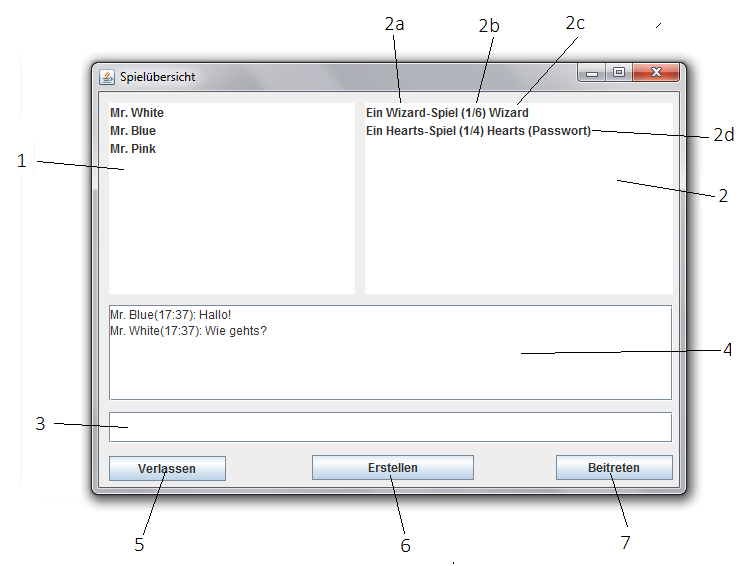
\includegraphics[width=\textwidth]{Lobby-Fenster}
\begin{itemize}
	\item \textbf{1) Spielerliste:} Hier sehen Sie Benutzernamen aller Spieler, die sich momentan in der \gls{Lobby}  befinden.
	\item \textbf{2) Spielliste:} Hier sehen Sie alle Spiele, die momentan noch auf Mitspieler warten oder noch nicht gestartet sind.
	\begin{itemize}
		\item \textbf{2a) Spielname:} Der Name des Spieles
		\item \textbf{2b) Spielerzahl:} Die Anzahl der momentanen Spieler/Die Anzahl der maximalen Spieler
		\item \textbf{2c) Regelwerk:} Welche Art von Spiel gespielt wird
		\item \textbf{2d) Passwort:} Zeigt an, ob der Beitritt zum Spiel passwortgeschüzt ist
		\item \textbf{2e) Gestartet:} Zeigt an, ob das Spiel bereits gestartet wurde. Ein Beitritt ist dann nicht mehr möglich
	\end{itemize}
	\item \textbf{3) Eingabefeld für den Chat:} In dieses Feld geben Sie ihre Chatnachrichten ein. Mit ENTER werden Sie versendet.
	\item \textbf{4) Chatverlauf:} Hier sehen Sie Ihre Chatnachrichten und die der anderen Nutzer.
	\item \textbf{5) Verlassen-Knopf:} Wenn Sie diesen Knopf drücken, wird die Anwendung beendet.
	\item \textbf{6) Erstellen-Knopf:} Drücken Sie diesen Knopf, wenn Sie ein neues Spiel erstellen wollen (mehr dazu in Kap. 5.4)
	\item \textbf{7) Beitreten-Knopf:} Wählen Sie ein Spiel in der Spieliste aus und drücken Sie auf diesen Knopf, um dem Spiel beizutreten. Ist das Spiel passwortgeschützt, erscheint folgendes Fenster, in welches Sie das Passwort eingeben müssen, um in das \gls{Wartefenster} zu gelangen.

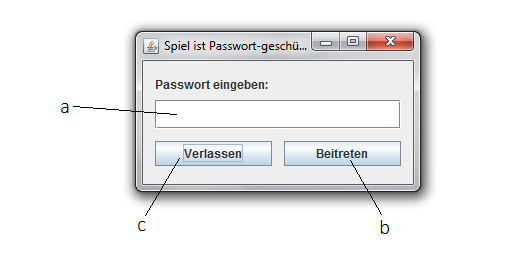
\includegraphics[width=\textwidth]{Passwort-Fenster}
\begin{itemize}
		\item \textbf{a) Passworteingabe:} Hier geben Sie das Passwort für das geschützte Spiel ein. Sollte es nicht mit dem gesetzten Passwort übereinstimmen, erhalten Sie eine Warnmeldung.
		\item \textbf{b) Beitreten-Knopf:} Drücken Sie auf diesen Knopf um das Passwort überprüfen zu lassen und dem Spiel beizutreten. Bei korrektem Passwort betreten Sie das \gls{Wartefenster} (siehe Kap. 5.4.2).
		\item \textbf{c) Verlassen-Knopf:} Die Texteingabe wird abgebrochen und Sie kehren in die \gls{Lobby} zurück.
\end{itemize}
\end{itemize}
\subsection{Spiel erstellen}
In der Lobby können Sie ein neues Spiel erstellen, indem Sie auf den Erstellen-Knopf (6)  drücken. Sie kommen in das \gls{Erstellungsfenster}.\\

\subsubsection{Erstellungsfenster}
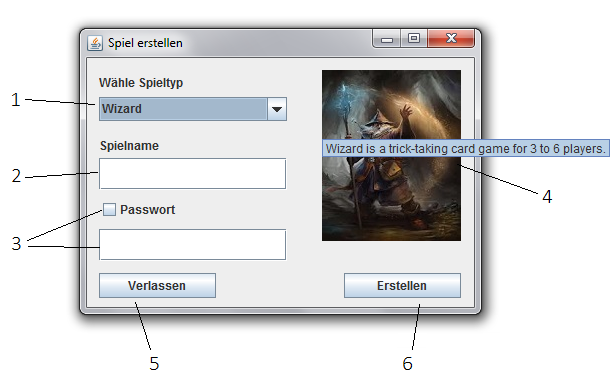
\includegraphics[width=\textwidth]{Erstellungs-Fenster}
\begin{itemize}
	\item \textbf{1) Spielauswahl:} Hier können Sie in einem Dropdown-Menü aus den\gls{Regelwerk}en Hearts oder Wizard auswählen
	\item \textbf{2) Eingabefeld für den Spielnamen:} Hier können Sie Ihrem Spiel einen Namen geben. Lassen Sie das Feld frei, so wird ein Standard Name für das Spiel gesetzt, bestehend aus Ihrem Benutzernamen + 's Spiel'.
	\item \textbf{3) Passwortschutz:} Wenn Sie in dem oberen Feld ein Häckchen setzen, können Sie den Zutritt zu Ihrem Spiel mit einem Passwort schützen, welches Sie in das untere Feld eingeben.
	\item \textbf{4) Spielbild:} Ein Bild passend zum\gls{Regelwerk}, welches Sie ausgewählt haben. Wenn Sie mit der Maus über das Bild fahren, erscheint eine Kurzbeschreibung zu diesem Spiel.
	\item \textbf{5) Verlassen-Knopf:} Wenn Sie diesen Knopf drücken, wird die Spielerstellung abgebrochen, und Sie kommen zurück in die Lobby.
	\item \textbf{6) Erstellen-Knopf:} Wenn Sie mit Ihren Einstellungen fertig sind, drücken Sie auf diesen Knopf, um das Spiel zu erstellen. Sie betreten das \gls{Wartefenster}, wo Sie auf den Beitritt von weiteren Spielern warten müssen, bis die Mindestzahl der Spieler erreicht ist, um das Spiel endgültig zu starten.	
\end{itemize}

\subsubsection{Wartefenster}
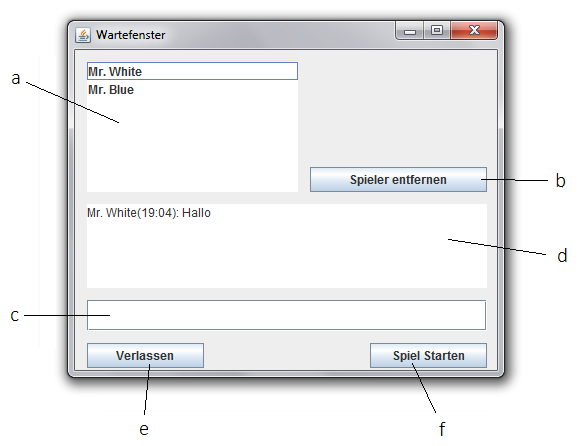
\includegraphics[width=\textwidth]{Warte-Fenster}
\begin{itemize}
	\item \textbf{a) Spielerliste:} Hier sehen Sie Benutzernamen aller Spieler, die sich momentan im \gls{Wartefenster} befinden.
	\item \textbf{b) Entfernen-Knopf:} Dieser Knopf ist nur für den Spielleiter sichtbar. Sie können damit andere Spieler aus dem \gls{Wartefenster} entfernen, die daraufhin wieder in die \gls{Lobby} zurückkehren. (Sie können sich nicht selbst aus dem \gls{Wartefenster} werfen. Bitte verwenden Sie den Verlassen-Knopf, wenn Sie in die \gls{Lobby} zurück möchten.)
	\item \textbf{c) Eingabefeld für den Chat:} In dieses Feld geben Sie Ihre Chatnachrichten ein. Mit ENTER werden Sie versendet.
	\item \textbf{d) Chatverlauf:} Hier sehen Sie Ihre Chatnachrichten und die der anderen Nutzer.
	\item \textbf{e) Verlassen-Knopf:} Mit diesem Knopf kehren Sie in die \gls{Lobby} zurück. Sollte der \gls{Spielleiter} das \gls{Wartefenster} verlassen, so wird das Spiel aufgelöst und alle Spieler werden in die Lobby zurück geschickt.
	\item \textbf{f) Start-Knopf:} Dieser Knopf ist nur für den \gls{Spielleiter} sichtbar. Sobald die Mindestanzahl an Spielern erreicht ist, kann damit das Spiel gestartet werden und das Spielfenster öffnet sich. (siehe Kap. 5.5)
\end{itemize}

\subsection{Spiel spielen}

Nachdem das Spiel im \gls{Wartefenster} gestartet wurde, befinden Sie sich nun im Spielfenster.\\
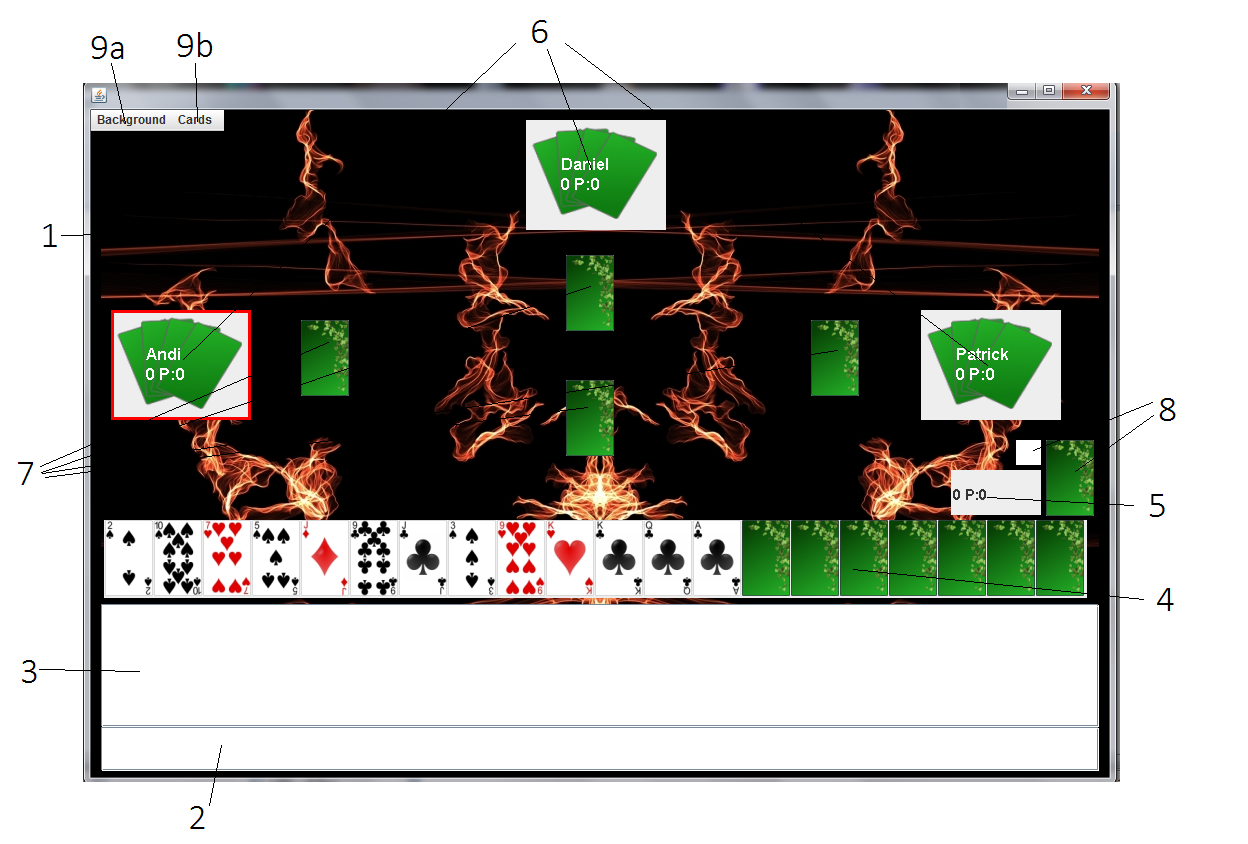
\includegraphics[width=\textwidth]{Spiel-Fenster}
\begin{itemize}
	\item \textbf{1) Spiefeld:} Hier läuft das Spiel ab.
	\item \textbf{2) Eingabefeld für den Chat:} In dieses Feld geben Sie ihre Chatnachrichten ein. Mit ENTER werden Sie versendet.
	\item \textbf{3) Chatverlauf:} Hier sehen Sie Ihre Chatnachrichten und die der anderen Nutzer.
	\item \textbf{4) Eigene Hand:} Hier sehen Sie Ihre eigenen Karten. Mit einem einfachen Klick wählen Sie eine Karte aus. Wenn Sie ein zweites Mal auf die markierte Karte klicken, spielen Sie diese.
	\item \textbf{5) Eigenes Anzeigefeld:} Hier sehen Sie je nach Regelwerk relevante Informationen über Ihren Punktestand bzw. Ihre gemachte Stiche.
	\item \textbf{6) Andere Spieler:} Es werden Informationen zu Ihren Mitspielern angezeigt.
	\item \textbf{7) Ablagestapel:} Hier sehen Sie die bereits gespielten Karten.
	\item \textbf{8) Aufnahmestapel:} Von diesem Stapel werden Karten gezogen. Beim Spiel Wizard sieht man daneben die Trumpffarbe.
	\item \textbf{9a) Hintergrundbild-Auswahl:} Hier können Sie ein Bild auswählen, das Sie als Hintergrundbild haben möchten.
	\item \textbf{9b) Hintergrundbild-Auswahl:} Hier können Sie das  Kartenhintergrudbild auswählen
\end{itemize}


\subsubsection{Wizard}

Wizard ist ein stichbasiertes Kartenspiel, bei dem es darum geht, die Stiche, die man pro Runde macht, so genau wie möglich vorherzusagen und so Punkte zu gewinnen. 
\begin{itemize}
	\item \textbf{Anzahl der Spieler:} 3-6 Spieler
	\item \textbf{Karten:}  60 Spielkarten (davon 52 :Blau, Rot, Grün, Gelb; Werte 1-13; sowie 8 Sonderkarten: 4 Zauberer und 4 Narren)
	\item \textbf{Auslegen:} Das Spiel wird in mehreren Partien gespielt, wobei die Anzahl von der Spielerzahl abhängt. In der ersten Partie erhält jeder Spieler eine Karte, in jeder weiteren Partie erhöht sich die Kartenanzahl, die jeder Spieler erhält, um eins. In der letzten Partie werden alle Karten gleichmäßig an die Spieler verteilt.
	\item \textbf{Spielende:} Das Spiel endet, sobald die letzte Partie gespielt wurde.
	\item \textbf{Spielverlauf:} Nachdem die Karten verteilt wurden, wird eine Karte auf dem Ablagestapel umgedreht, die die \gls{Trumpf}farbe angibt. Wird ein Zauberer umgedreht, so bestimmt der ausgebende Spieler die \gls{Trumpf}farbe.
	\begin{itemize}
		\item \textbf{Stichansage:} Zu Beginn jeder Partie müssen die Spieler schätzen, wie viele Stiche sie in dieser machen werden.
		\item \textbf{Spiel:} Im Uhrzeigersinn werden Karten gespielt. Dabei herrscht \gls{Farbzwang}.Allerdings kann eine weiße Karte (Zauberer oder Narr) unabhängig davon, immer gespielt werden. War die erste Karte ein Narr, so entscheidet die nächste farbige Karte, welche Farbe gespielt werden muss. War die erste Karte ein Zauberer, so kann jeder Spieler eine beliebige Karte spielen. Nach einer \gls{Spielrunde} erhält der Spieler mit der höchsten Karte den Stich. Dabei gilt:
		\begin{enumerate}
			\item Der erste gespielte Zauberer sticht über alle anderen Karten.
			\item Ist kein Zauberer gespielt worden, so sticht der höchste \gls{Trumpf} über die anderen Karten.
			\item Ist kein Zauberer und kein \gls{Trumpf} gespielt worden, so bekommt derjenige Spieler den \gls{Stich}, der die höchste Karte der geforderten Farbe gespielt hat.
			\item Ein Narr macht keinen \gls{Stich}, es sei denn, in einem \gls{Stich} werden nur Narren gespielt. In diesem Fall 'gewinnt' der erste Narr den Stich.
		\end{enumerate}
	\end{itemize}
	\item \textbf{Punkteauswertung:} Stimmt die Anzahl der gemachten Stiche mit der Anzahl der vorhergesagten Stiche überein, so bekommt der Spieler 20 Punkte für die richtige Prognose sowie 10 Punkte für jeden Stich. Stimmt sie nicht überein, bekommt er für jeden Stich Abweichung 10 Minuspunkte. Gewinner ist derjenige mit den meisten Punkten am Ende des Spiels.
\end{itemize}
\subsubsection{Hearts}
Hearts ist ein stichbasiertes Kartenspiel, bei dem es darum geht, so wenig Punkte wie möglich zu machen.
\begin{itemize}
	\item \textbf{Anzahl der Spieler:} 4 Spieler
	\item \textbf{Karten:}  52 Spielkarten (Kreuz, Pik, Herz, Karo; 2–10, Bube/Bauer, Dame, König, Ass)
	\item \textbf{Auslegen:} Die Karten werden gleichmäßig an alle Spieler verteilt. Jeder erhält 13 Karten.
	\item \textbf{Spielende:} Sobald ein Spieler 100 Punkte erreicht hat, endet das Spiel.
	\item \textbf{Spielverlauf:}
	\begin{itemize}
		\item \textbf{Kartentausch:} Zu Beginn der ersten \gls{Partie} wählt jeder Spieler drei Karten aus und gibt Sie seinem linken Nachbarn. In der zweiten \gls{Partie} werden die drei Karten nach rechts gegeben. In der dritten \gls{Partie} werden drei Karten mit dem Gegenüber getauscht. In der vierten \gls{Partie} wird nicht getauscht. Danach beginnt es wieder von vorne.
		\item \textbf{Spiel:} Der Spieler, der die Kreuz 2 auf der Hand hat, beginnt die \gls{Partie}, indem er diese legt. Im Uhrzeigersinn müssen die anderen Spieler nun Karten dazugeben. Dabei herrscht \gls{Farbzwang}. Außerem darf im ersten Zug weder Herz noch die Pik Dame gelegt werden, es sei denn der Spieler hat nichts anderes auf der Hand. Wenn die \gls{Spielrunde} vorbei ist, erhält der Spieler den \gls{Stich}, der die höchste Karte in der Farbe der zuerst ausgespielten Karte gespielt hat. Der Spieler, der den \gls{Stich} gemacht hat eröffnet die nächste \gls{Spielrunde}, indem er eine Karte legt. Diese darf nur dann eine Herzkarte sein, wenn zuvor eine Herzkarte ausgespielt wurde.
	\end{itemize}
	\item \textbf{Punkteauswertung:} Nach einer \gls{Partie} werden die Punkte der \gls{Stich}e gezählt. Pro Herz gibt es einen Punkt und für die Pik Dame 13 Punkte. Hat ein Spieler in einer \gls{Partie} alle Herzkarten sowie die Pik Dame gesammelt, so erhalten seine Mitspieler 26 Punkte und er selbst 0. Die Punkte pro Partie werden aufsummiert. Gewinner ist derjenige mit den wenigsten Punkten am Ende des Spiels.
\end{itemize}

\section{Fehlermeldungen und Behebung}
Tritt ein Fehler auf, werden Sie durch eine entsprechende Fehlermeldung gewarnt.
Die folgende Auflistung einiger Fehler hilft Ihnen bei der Behebung:
\begin{itemize}
\item \textbf{Fehler Server}:
	\begin{itemize}
	\item \textbf{Fehler beim Start}:
		Sollte der gewählte Port bereits belegt sein, bekommen Sie eine Fehlermeldung, bitte wählen Sie in diesem Fall einen anderen Port.
		{Fehler beim der Verbindung}:
		Sollten Sie selbst den Server gestartet haben und keine Verbindung möglich sein, überprüfen Sie bitte, ob das Programm wirklich läuft und ob ihr Port freigegeben wurde.
	\end{itemize}
\item \textbf{Fehler Client}:
	\begin{itemize}
	\item \textbf{Fehler bei der Verbindung}:
		Sollte die Verbindung plötzlich beendet werden, müssen Sie das Spiel neu starten (siehe 5.1 Spielstart). Sollten Sie bereits in einem Spiel gewesen sein, wurde das Spiel beendet und ihre Mitspieler befinden sich wieder in der Lobby.
	\item \textbf{Fehler beim Login}:
		\begin{itemize}
		\item \textbf{Fehler bei der Namenseingabe}:
			Tritt hier ein Fehler auf, erhalten Sie eine Fehlermeldung. In diesem Fall sollten Sie einen anderen Namen wählen, da der zuvor gewählte bereits vergeben ist.
		\item \textbf{Fehler beim Verbindungsaufbau}:
			Sollte der gewählte Port bereits belegt sein, bekommen Sie eine Fehlermeldung, bitte wählen Sie in diesem Fall einen anderen Port.
Sollte die gewählte IP Adresse nicht korrekt sein, d.h. auf dem Rechner mit dieser IP wurde kein Server gestartet, so erhalten Sie eine Fehlermeldung. Überprüfen Sie dann bitte ihre Eingabe auf Richtigkeit oder wählen Sie eine andere IP-Adresse.
Die Adresse kann auf folgende Weisen angegeben werden: \\
IP-Adresse\\
servername.de:port\\
ip:port\\
		\end{itemize}
	\end{itemize}
\end{itemize}

\section{Entwicklung eines neuen \gls{Regelwerk}es}
Die Anwendung NET-WizHearts ist so konzipiert, dass jederzeit weitere \gls{Regelwerk}e hinzugefügt werden können.
Dazu ist die Entwicklung folgender Klassen notwendig:
\begin{itemize}
\item \textbf{Paket Ruleset}
	\begin{itemize}
	\item \textbf{Neue Klassen}:
		\begin{itemize}
		\item \textbf{Server''NameOfTheGame''}: Diese Klasse erbt von ServerRuleset. Es ist eine Klasse, die die Einhaltung der Regeln garantiert - Serverseitig.
		\item \textbf{Client''NameOfTheGame''}: Diese Klasse erbt von ClientRuleset. Dies ist eine Klasse, die eine Vorab-Regelauswertung vornehmen soll- Clientseitig.
	
		 Achten Sie bei der Entwicklung dieser Klassen darauf, dass die Methode isValidMove in beiden oben genannten Klassen den selben Inhalt hat! Andernfalls wertet der Server dies als Betrugsversuch eines Spielers und dieser wird aus dem Spiel geworfen.
		 \item \textbf{''NameOfTheGame''Card}: Neue Klasse, die alle Karten enthalten muss, die für das Regelwerk benötigt werden.
		\item \textbf{''NameOfTheGame''Data}: Neue Klasse, die die Otherdata eines Spielers zum Regelwerk enthält.
	\end{itemize}
	\item \textbf{Änderungen an bestehenden Klassen}:
		\begin{itemize}
		\item \textbf{RulesetType}: Eine Änderung dieser Klasse ist unbedingt nötig. Fügen sie dazu den Namen des entsprechenden Regelwerkes mit der Mindest- und Höchstspielerzahl ein.
		\item \textbf{Color}: Eventuelle Änderungen in dieser Klasse, sollten andere Farben für das neue Regelwerk benötigt werden. Fügen Sie einfach die Namen der Farben in die schon bestehende Auflistung hinzu.
		\item \textbf{GamePhase}: Eventuelle Änderungen in dieser Klasse, sollten die bereits existierenden Phasen nicht ausreichen. Benötigen Sie eine Spielphase, die noch nicht existiert, so fügen Sie diese einfach in die bereits bestehende Auflistung hinzu.
		\item \textbf{UserMessages}: Eventuelle Änderungen an dieser Klasse, sollten die bereits existierenden Nachrichtentypen nicht ausreichen. Fügen Sie diese einfach in die bereits bestehende Auflistung hinzu.
		\end{itemize}
	\end{itemize}
\item \textbf{Data:} Sollten Sie neue Bilder/Daten benötigen, fügen Sie diese bitte in den Ordner 'Data' ein. Für neue Karten, erstellen Sie bitte einen neuen Ordner.
\end{itemize}

\newpage
\printglossaries

\end{document}